%% AMS-LaTeX Created by Wolfram Mathematica 9.0 : www.wolfram.com

\documentclass{article}
\usepackage{amsmath, amssymb, graphics, setspace}
\usepackage{graphicx}

\usepackage[utf8]{inputenc}
\usepackage{spverbatim}
\usepackage{geometry}
 \geometry{
 a4paper,
 left=15mm,
 right=10mm,
 top=20mm,
 bottom=20mm,
 }



\newcommand{\mathsym}[1]{{}}
\newcommand{\unicode}[1]{{}}

\newcounter{mathematicapage}
\begin{document}


\section{Ondas de sonido}
Una perturbación de pequeña amplitud en un fluido va a crear zonas de compresión y rarefacción que alternan en el tiempo y espacio en la dirección de propagación(el movimiento oscilatorio de las particulas se propaga como una onda y son ondas logitudinales:  las particulas se mueven en la misma dirección que la dirección de propagación)

\paragraph{Condiciones iniciales}
Consideramos un fluido ideal con las variables en el estado de equilibrio $v_0 = 0, \rho_0 , p_0$ y hacemos unos cambios en estas variables que  son muy pequeños de forma que se pueden omitir los términos de segundo orden (o mayores) en las ecuaciones de los fluidos
Definimos $c_s = \big( \frac{\partial p}{\partial \rho}\big)_s = \sqrt{\gamma \frac{p_0}{\rho_0}}$
Las variables de cuales queremos estudiar la evolución devienen:

\begin{description}  
\item v
\item $\rho = \rho_0 + \rho_0\prime$
\item $p = p_0 + p\prime$

 
\end{description}  

con $|v|<<c_s, p\prime<<p , \rho\prime << \rho_0$ 

Las ecuaciones de los fluidos despues de linearlizar devienen:
\begin{description}  
\item continuidad: $ \frac{\partial \rho\prime}{\partial t} + \rho_0 \nabla \cdot v = 0 $
\item Euler: $ \frac{\partial v}{\partial t} + \frac{1}{\rho_0} \nabla p\prime = 0 $

\end{description}  

\begin{description}  
\item El proceso es adiabático: $p\prime = c_s^{2} \rho\prime$

\item Después de hacer los cálculos (y suponiendo el caso general inhomogeneo en tiempo y espacio : $\rho_0 = \rho_0(x,t) \implies c_s = c_s(x,t)$ con la densidad de equilibrio variando bastante lentamente en el espacio y tiempo de tal forma que se pueden omitir terminos de segundo orden o mas en multiplicaciones de derivadas temporales o espaciales de estas y las perturbaciones) las perturbaciones de las variables verifican las ecuaciones: 

\item $\frac{\partial}{\partial t} \big(\frac{1}{c_s^{2}(x,t)} \frac{\partial p\prime}{\partial t}\big) = \nabla^{2} p\prime    $
\item $\frac{\partial}{\partial t} \big(\frac{1}{c_s^{2}(x,t)} \frac{\partial \rho\prime}{\partial t}\big) = \nabla^{2} \rho\prime    $
\item $\frac{\partial}{\partial t} \big(\frac{1}{c_s^{2}(x,t)} \frac{\partial \Phi}{\partial t}\big) = \nabla^{2} \Phi $ donde definimos  $v = \nabla \Phi$ considerando el fluido irrotacional
\item Si la densidad de equilibrio no varia en el tiempo($\rho_0 = \rho_0(x)$):
\item $\frac{1}{c_s^{2}(x)} \frac{\partial^{2} p\prime}{\partial t^{2}} = \nabla^{2} p\prime    $
\item $\frac{1}{c_s^{2}(x)} \frac{\partial^{2} \rho\prime}{\partial t^{2}} = \nabla^{2} \rho\prime    $
\item $\frac{1}{c_s^{2}(x)} \frac{\partial^{2} \Phi}{\partial t^{2}} = \nabla^{2} \Phi    $
\end{description}  

\paragraph{Medio homogeneo}

\begin{description}  
\item Si la densidad de equilibrio es constante en tiempo($\rho_0, c_s constantes$) y espacio las soluciones generales son superposiciones de ondas planas de forma:
\item $ \sum_{i} A_{\rho\prime_i} cos (x - c_s t) $
\item $ \sum_{i} A_{p\prime_i} cos (x - c_s t) $
\item $ \sum_{i} csSign_i A_{v_i} cos (x - csSign_i c_s t) $ donde $csSign_i = 1 $ si la onda viaja a la derecha y -1 si va a la izquierda
\item con las amplitudes números reales verificando las ecuaciones:
$A_{p\prime_i} = c_s^{2} A_{\rho\prime_i}$
$A_{v_i} = \frac{1}{c_s \rho_0} A_{p_i}$
\end{description}  


\paragraph{Medio inhomogeneo} $\rho_0 = \rho_0(x)$
La solución no se puyede expresar mas como superposición de ondas planas (porque $c_s$ no es más constante ), pero análogo a esta solución intentamos  buscar soluciones de forma $a(x,t) e^{i\phi(x,t)}$ (aproximación WKB):
 donde definimos 
\begin{description}  
\item $\omega(x,t) = -\frac{\partial \phi}{\partial t}$
\item $k(x,t) = -\nabla \phi$
\end{description}
porque análogo al caso homogeneo (considerando sin perder la generlaidad solo una onda y no una superposición) donde $\phi(x,t) = kx-\omega t$ con $\omega, k$ constantes verificando la relación de dispersión $\omega^{2} = c_s^2 k^2  $  

\textbf{Relación entre las amplitudes}

\begin{description}  
\item Suponiendo que estas soluciones existen:
\item $p\prime = P e^{i\phi}$
\item $\rho\prime = R e^{i\phi}$
\item $v = V e^{i\phi}$
\item P,R,V  complejos
\end{description}

igual que en caso homogeneo :

\begin{description}  
\item de la relación de adiabaticidad: $|P(x,t)| = c_s^{2}(x) |R(x,t)|$
\item de la ecuación de movimiento: 
\item $\rho_0 \frac{\partial v}{\partial t} = -\nabla \rho\prime \implies -i \rho_0 \omega V e^{i\phi} = i k P e^{i\phi}$
\item despues de simplificar,  multiplicar cada lado con su conjugado(hay que expresar las amplitudes locales con el módulo porque pueden ser complejas):
\item  $|V|^2 = \frac{|P|^2}{\rho_0^{2} c_s^2}$ ($|V|= \frac{1}{c_s \rho_0} |P| = \frac{c_s}{p_0 \gamma} |P|$) 


\end{description}

\paragraph{Resolver la ecuación genérica}
\begin{description}  
\item $\frac{1}{c_s^{2}(x)} \frac{\partial^{2} p\prime}{\partial t^{2}} = \nabla^{2} p\prime    $
\item Reemplazando la solución WKB approx. $p(x,t) = a(x,t) e^{i \phi(x,t)}$ en la ecuación y con las definiciones de $\omega$ y k de arriba despues de hacer los cálculos 
\item $\omega^{2}(x,t) = c_s^{2}(x) k^2(x,t)$
\item definiendo $c_g = \frac{\partial \omega}{\partial k}$ :
\item $\frac{\partial a}{\partial t} + c_g \cdot \nabla a = -\frac{1}{2} \frac{a}{|k| c_s} (\frac{\partial \omega}{\partial t} + c_s^{2} \cdot \nabla k) $

\item $\implies $ 
\item$\frac{\partial \omega}{\partial t} + c_g \cdot \nabla \omega = 0 $
\item$\frac{\partial k}{\partial t} + c_g \cdot \nabla k = -k \cdot \nabla c_g $

\item Usamos directamente la ecuación de conservación de energía para determinar la amplitud:
\item$\frac{\partial E}{\partial t} + c_g \cdot \nabla E = -E \nabla \cdot c_g $

\end{description}


\textbf{1D} ($c_s = c_g$):
\begin{description}  
\item $\frac{1}{c_s^{2}(x)} \frac{\partial^{2} p\prime}{\partial t^{2}} = \nabla^{2} p\prime    $
\item$\frac{\partial k}{\partial t} + c_s \frac{\partial k}{\partial x} = -c_s $
\item$\frac{\partial \omega}{\partial t} + c_s \frac{\partial \omega}{\partial x} = 0 $
\item$\frac{\partial k}{\partial t} + c_s \frac{\partial k}{\partial x} = -k \frac{\partial c_s}{\partial x} $
\item$\frac{\partial E}{\partial t} + c_s \frac{\partial E}{\partial x} = -E \frac{\partial  c_s}{\partial x} $


\end{description}

Al largo de un rayo definido por:

\begin{description}  
\item$\frac{dx}{dt} = c_s $
\item$ x_p(t) , x_p(0) = x_p $
\end{description}

las funciones:
\begin{description}  
\item $\omega_p(t) = \omega(x_p(t), t)$
\item$k_p(t) = k(x_p(t), t)$
\item$a_p(t) = a(x_p(t), t)$
\end{description}

verifican las ecuaciones
\begin{description}  
\item $\frac{d\omega_p}{dt} = 0$
\item $\frac{dk_p}{dt} = -k_p \frac{\partial c_s}{\partial x} (x_p(t))$
\item $\frac{dc_s}{dt}  =  \frac{\partial c_s}{\partial x}(x_p(t)) c_s$
\end{description}

\begin{description}  
\item $\frac{dk_p}{dt} = -k_p  \frac{1}{c_s} \frac{dc_s}{dt} \implies$
\item $\frac{dln(k_p)}{dt} = - \frac{dln(c_s)}{dt} \implies $
\item $ k(x_p(t), t)  c_s(x_p(t)) = constant $
\item de forma similar $ E(x_p(t), t)  c_s(x_p(t)) = constant $ 
\item $ \omega(x_p(t), t)  = constant $
\end{description}

Ecuación de la energía:
\begin{description}  

\item $\frac{\rho_0 |V|^{2}}{2} = \frac{|P|^{2}} {2 \rho_0 c_s^{2}} $
\item $E = \frac{|P|^{2}}{\rho_0 c_s^2} $ (la suma de las 2)
\item $\implies |P(x_p(t),t)| c_s^{\frac{1}{2}}(x_p(t),t) = constant $
\end{description}

\begin{description}  
\item Suponemos que podemos escribir :
\item $|P| = c_s^{k} \rho_0^{l} p_0^{m} C_{P}$
\item $|R| = c_s^{k} \rho_0^{l_1} p_0^{m_1} C_{R}$
\item $|V| = c_s^{k} \rho_0^{l_2} p_0^{m_2} C_{V}$
\item con $C_{P}, C_{R} y C_{V}$ constantes. Estas relaciones serían válidas aunque $p_0$ no es constante? (TODO: variando de tal forma que se cumplan las condiciones de las aproximaciones : $\rho_0, p_0, c_s$ monotonas variando lentamente)
\item de las relaciones entre las amplitudes de arriba 
\item $\frac{|P|}{|R|} = c_s^2 = \rho_0^{l-l_1} p_0^{m-m_1} \frac{C_{P}}{C_{R}}$
\item Escribimos $c_s^2 = \gamma p_0 \rho_0^{-1}$ y la relación de arriba se tiene que cumplir $\forall x$ (porque consideramos $c_s, \rho_0 y p_0 $ dependiendo de x)
\item $\implies m - m_1 = 1$, $l-l_1 = -1$ y $\frac{C_P}{C_R} = \gamma$
\item $\frac{|P|}{|V|} = c_s \rho_0 = \gamma^{-\frac{1}{2}} p_0^{\frac{1}{2}} \rho_0^{\frac{1}{2}} = \rho_0^{l-l_2} p_0^{m-m_2} \frac{C_P}{C_V}$
\item $\implies  \frac{C_P}{C_V} =  \gamma^{-\frac{1}{2}}, l-l_2=\frac{1}{2}. m-m_2 = \frac{1}{2} $
\item Para determinar la relación entre m,l,k introducimos en la ecuación de la energia la expresion de $|P|$
\item $ c_s^{2k} \rho_0^{2l} p_0^{2m} \rho_0^{-1} c_s^{-2} c_s  $ tiene que ser constante al largo del rayo
\item Reemplazano $c_s$ : $ \gamma^{k + \frac{1}{2}} p_0^{k-\frac{1}{2}+2m} \rho_0^{-k + 2l -\frac{1}{2}} $ tiene que ser constante al largo del rayo (eligiendo un punto inicial y $\forall t$)
\item $\implies k = 2l - \frac{1}{2} = \frac{1}{2} - 2m$ y $2m + 2l = 1$
\item elegimos $k = l = \frac{1}{2}$ , $m = 0$ (TODO eso porque en realidad se puede dejar un parámetro ya que $\gamma = const = c_s^{2} \rho_0^{-1} p_0^{-1} $ y multiplicando las ecuaciones con $\gamma^{p}$ el parámtro $m\rightarrow m+p$ ? o hay que elegir porque todas las amplitudes tienen que cumplir la ecuación diferencial de la amplitud?)
\item $\implies m_1=-1, l_1 = \frac{3}{2}, l_2 = 0, m_2 = -\frac{1}{2}$
 
\item $|P| = c_s^{\frac{1}{2}} \rho_0^{\frac{1}{2}}  C_{P}$
\item $|R| = c_s^{\frac{1}{2}} \rho_0^{\frac{3}{2}} p_0^{-1} \gamma^{-1} C_{P}$
\item $|V| = c_s^{\frac{1}{2}}  p_0^{-\frac{1}{2}} \gamma^{\frac{1}{2}} C_{P}$

\item Las amplitudes se calculan al largo del rayo (en la curva determinada por $\frac{dx}{dt} = c_g, x(0) = x_p$): $C_P$ es una constante que depende de los valores en el punto inicial del rayo ($x_p$): $C_P = c_s^{-\frac{1}{2}}(x_p) , \rho_0^{\frac{1}{2}}(x_p)$

\item En el caso de la práctica (con $p_0$ constante ) queremos representar las amplitudes como $const * cs^{\alpha} $ reemplazamos $\rho_0$
y calculanido al largo del rayo  $\frac{dx}{dt} = c_g, x(0) = x_p$:
\item $|P(x_p(t),t)| = c_s^{-\frac{1}{2}}(x_p(t)) c_s^{\frac{1}{2}}(x_p) P(x_p,0)  $ (sé en cada momento en cada punto que punto incial en el rayo le corresponde)
\item las amplitudes de las demás perturbaciones se calculan reemplazando directamente en las relaciones entre las amplitudes (cuando se representa la solución analítica), 
\item Para ver si el paquete se adapta a la relación representamos las curvas:
\item para la presión: $ c_s^{-\frac{1}{2}}(x) c_s^{\frac{1}{2}}(x) P(x_0,0) $
\item densidad: $ c_s^{-\frac{3}{2}}(x) c_s^{\frac{3}{2}}(x_0) R(x_0,0)  $ 
\item velocidad: $ c_s^{\frac{1}{2}}(x) c_s^{-\frac{1}{2}}(x_0) V(x_0,0)  $ 
\item eligiendo $x_0$ los 2 puntos donde  los valores de las amplitudes de las perturbación en el momento inicial tienen el mínimo y máximo de 


\end{description}



\section{Transf fourier}

Salida de mathematica de la integral de la transf fourier:

\begin{spverbatim}

$Assumptions = {Element[{k0,z0,zf,zc,W}, Reals], k0>0, z0>0, zf >0 , zf >0, zc >0, W>0 }
Print[FullSimplify[Integrate[Exp[- (z-zc)^2 / W^2] Cos[2 Pi  k0 (z - z0)/ (zf - z0)] Exp[- 2 Pi I m z / (zf - z0)],  {z, -Infinity, Infinity} ]]]

\end{spverbatim}

$
f1(m)=F( \frac{2\pi m}{z_f - z_0} ) = \int_{- \infty}^{\infty}{e^{-\frac{(z-z_c)^2}{W^2}} cos(\frac{2 \pi k_0 (z-z_0)}{z_f - z_0}) e^{-\frac{2 \pi i m z }{z_f - z_0}} dz } = $

$\frac{1}{2} e^{-\frac{\pi  \left(\text{$k_0$}^2 \pi  W^2+m \left(m \pi  W^2-2 i \text{$z_c$} (\text{$z_0$}-\text{$z_f$})\right)+2 \text{$k_0$} \left(m \pi  W^2+i
(\text{$z_0$}+\text{$z_c$}) (\text{$z_0$}+\text{$z_f$})\right)\right)}{(\text{$z_0$}-\text{$z_f$})^2}} \left(e^{\frac{4 i \text{$k_0$} \pi  \text{$z_0$} (\text{$z_c$}+\text{$z_f$})}{(\text{$z_0$}-\text{$z_f$})^2}}+e^{\frac{4
\text{$k_0$} \pi  \left(m \pi  W^2+i \left(\text{$z_0$}^2+\text{$z_c$} \text{$z_f$}\right)\right)}{(\text{$z_0$}-\text{$z_f$})^2}}\right) \sqrt{\pi } W$


Salida de FourierTransform mathematica con FourierParameters 0, -2$\pi$ 

\begin{verbatim}

$Assumptions = {Element[{k0,z0,zf,zc,W}, Reals], k0>0, z0>0, zf >0 , zf >0, zc >0, W>0 }
h[z_, k0_, z0_, zf_, zc_, W_]:= Exp[-(z-zc)^2/W^2] Cos[2 Pi k0 (z - z0) / (zf - z0) ]
Print[FullSimplify[FourierTransform[h[z, k0, z0, zf, zc, W], z, k, FourierParameters->{0,-2 Pi}]] ]

\end{verbatim}
$f2(k)=$

$\frac{1}{2} \left(e^{-\frac{\pi  \left(\text{$k_0$}^2 \pi  W^2-2 \text{$k_0$} \left(k \pi  W^2-i \text{$z_0$}+i \text{$z_c$}\right) (\text{$z_0$}-\text{$z_f$})+k
\left(k \pi  W^2+2 i \text{$z_c$}\right) (\text{$z_0$}-\text{$z_f$})^2\right)}{(\text{$z_0$}-\text{$z_f$})^2}}+ \\
e^{-\frac{\pi  \left(\text{$k_0$}^2 \pi  W^2+2 \text{$k_0$}
\left(k \pi  W^2-i \text{$z_0$}+i \text{$z_c$}\right) (\text{$z_0$}-\text{$z_f$})+k \left(k \pi  W^2+2 i \text{$z_c$}\right) (\text{$z_0$}-\text{$z_f$})^2\right)}{(\text{$z_0$}-\text{$z_f$})^2}}\right)
\sqrt{\pi } W$

En esta reemplazo k = k / (zf - z0) y los graficos salen iguales ($f1(k) = f2(\frac{k}{z_f - z0})$)


Ademas la salida de:
\begin{spverbatim}
$Assumptions = {Element[{k0,z0,zf,zc,W}, Reals], k0>0, z0>0, zf >0 , zf >0, zc >0, W>0 }

f1[m_]:=((E^(((4*I)*k0*Pi*z0*(zc + zf))/(z0 - zf)^2) + E^((4*k0*Pi*(m*Pi*W^2 + I*(z0^2 + zc*zf)))/(z0 - zf)^2))*Sqrt[Pi]*W)/
  (2*E^((Pi*(k0^2*Pi*W^2 + m*(m*Pi*W^2 - (2*I)*zc*(z0 - zf)) + 2*k0*(m*Pi*W^2 + I*(z0 + zc)*(z0 + zf))))/(z0 - zf)^2))
f2[k_]:=((E^(-((Pi*(k0^2*Pi*W^2 - 2*k0*(k*Pi*W^2 - I*z0 + I*zc)*(z0 - zf) + k*(k*Pi*W^2 + (2*I)*zc)*(z0 - zf)^2))/(z0 - zf)^2)) +
      E^(-((Pi*(k0^2*Pi*W^2 + 2*k0*(k*Pi*W^2 - I*z0 + I*zc)*(z0 - zf) + k*(k*Pi*W^2 + (2*I)*zc)*(z0 - zf)^2))/(z0 - zf)^2)))*Sqrt[Pi]*W)/2

Print[FullSimplify[f1[k]-f2[k/(zf-z0)]]]

\end{spverbatim}

es 0


Elijo f2 forma para simplificar (después de hacer los gráficos de los modulos de los valores de la función , tal como imaginaba la primera exponencial corresponde a la gaussiana de las frecuancias negativas y la segunda de las frequencias positivas):


$f1(k) = f2(\frac{k}{(z_f - z_0)}) = $

$ \frac{W \sqrt{\pi}}{2}  (e^{-\frac{\pi (k_0^2 \pi  W^2 + 2 k_0 k \pi W^2 + 2 k_0 i  (z_c - z_0) (z_f-z_0)+k^2 \pi W^2 +
2 i k z_c (z_f - z_0))}{(z_0-z_f)^2}}+e^{-\frac{\pi  (k_0^2 \pi  W^2 - 2 k_0 k \pi  W^2 - 2 k_0 i (z_c - z_0) (z_f-z_0)+k^2 \pi  W^2+2 i k z_c (z_f - z_0))}{(z_0-z_f)^2}}) =
$

$ \frac{W \sqrt{\pi}}{2}  (e^{-\frac{\pi \big[ \pi  W^2 (k + k_0)^2   + 2 k_0 i z_c(z_f - z_0)   - 2 k_0 i z_0 (z_f-z_0) +
2 i k z_c (z_f - z_0)\big]}{(z_0-z_f)^2}}+e^{-\frac{\pi \big[\pi  W^2 (k - k_0)^2  -2 k_0 i z_c(z_f - z_0)  + 2 k_0 i z_0 (z_f-z_0)+2 i k z_c (z_f - z_0)\big]}{z_0-z_f)^2}}) =
$

$ \frac{W \sqrt{\pi}}{2}  (e^{-\frac{\pi \big[ \pi  W^2 (k + k_0)^2   + 2  i z_c(z_f - z_0)(k_0 + k)   - 2 k_0 i z_0 (z_f-z_0) \big]}{(z_0-z_f)^2}}+e^{-\frac{\pi \big[\pi  W^2 (k - k_0)^2  +2 i z_c(z_f - z_0)(k - k_0)  + 2 k_0 i z_0 (z_f-z_0)\big]}{(z_0-z_f)^2}}) =
$

Considerando $z_c$ = 0 
las exponenciales son  gaussianas  con w = $\frac{z_f - z_0}{\pi W}$ la primera centrada en $-k_0$ y la segunda en $k_0$
y cuando calculamos el modulo las constantes $ abs(exp( - 2 k_0 i z_0 (z_f-z_0))) = abs(exp( 2 k_0 i z_0 (z_f-z_0)))  = 1$
y la amplitud queda $\frac{W \sqrt{\pi}}{2}$ igual que se ve en el gráfico (con valores :  z0=3.100, zf = 7.400, k0 = 60, zc = 3.745, W = 0.050) : con rojo había hecho el plot de la función entera y con verde y azul de las 2 partes al principio para estar segura que correspondían a las 2 partes

\begin{figure}[!ht] 
 \centering 
 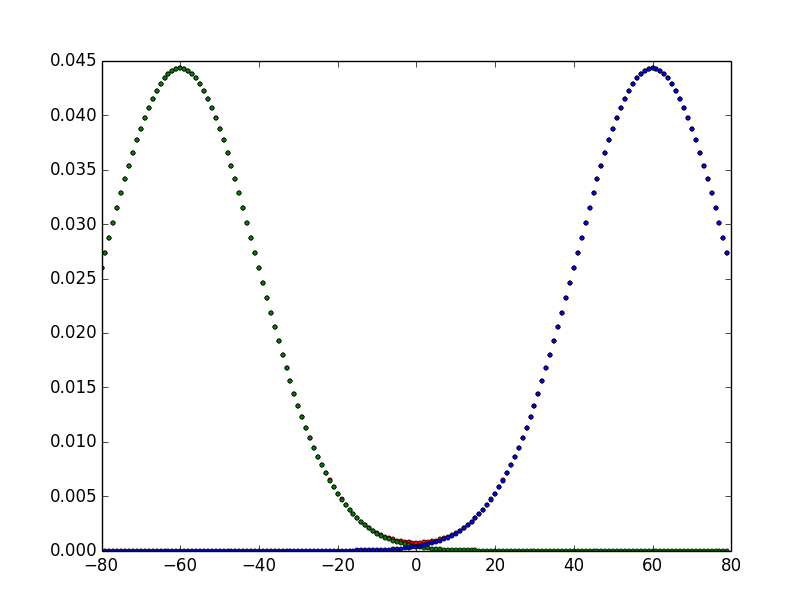
\includegraphics[scale=0.5]{gauss.png} 
\end{figure} 
 

\end{document}


